%% The following is a directive for TeXShop to indicate the main file
%%!TEX root = diss.tex

\chapter{Introduction}
\label{ch:Introduction}

%%%%%%%%%%%%%%%%%%%%%%%%%%%%%%%%%%%%%%%%%%%%%%%%%%%%%%%%%%%%%%%%%%%%%%
\section{Motivation}
\label{sec:Motivation}

Since the neutrino was first postulated by Wolfgang Pauli in 1930 \cite{neutrinoHistory}, investigation into their properties has presented a significant challenge for physics researchers, with a great impact on our understanding of the universe.
Because neutrinos do not react via the electromagnetic force, they may only be detected via the weak force.

There are three flavors of neutrinos: the electron neutrino $\nu_e$, the muon neutrino $\nu_\mu$, and the tau neutrino $\nu_\tau$.
In 1998, the Super-Kamiokande detector in Japan observed clear evidence of neutrino oscillation: as neutrinos of one flavor travels over a large distance, it has some probability of later being observed as a neutrino of another generation.
This implied that neutrinos have a nonzero mass, a result not predicted by the Standard Model.
The theorized explanation for neutrino oscillation is that each neutrino flavor actually exists as some superposition of 3 different mass states - as a neutrino travels over large distances, the differences in phases of the mass states results in a shifting probability of detecting each neutrino flavor.
The relationship between mass and flavor states is governed by the following relation:

\[
\begin{pmatrix}
\nu_e \\ \nu_\mu \\ \nu_\tau
\end{pmatrix}
=
U \begin{pmatrix}
\nu_1 \\ \nu_2 \\ \nu_3
\end{pmatrix}
\]

Here, U is a $3 \times 3$ unitary matrix, known as the PMNS Matrix.
The matrix can be characterized by 4 parameters: $\theta_{12}, \theta_{23}, \theta_{13}$, which are the "mixing angles", and $\delta_{CP}$, known as the CP-violating phase \cite{pdg2018}. 

There are many open-ended questions regarding neutrinos.
The parameters of the PMNS Matrix are poorly constrained.
% TODO: SEPARATE OUT SENTENCES FOR EACH LINE AFTER THIS
The neutrino masses are currently unknown, nor is it known why their masses are so small, nor are the mass orderings of the three states known.
It is unknown whether neutrinos are their own anti-particles (i.e. whether the neutrino is a Majorana fermion), or if the antineutrino is a distinct particle (i.e. a Dirac fermion). It is uncertain whether the $\delta_{CP}$ is consistent with zero: If it is nonzero, then that may explain the asymmetry between the amount of matter and antimatter in the universe \cite{neutrinoCP}.

The Super-Kamiokande experiment that first observed neutrino oscillations did so by observing atmospheric neutrinos: upon collision with atoms in the earth's atmosphere, energetic cosmic rays produce a shower of secondary particles such as pions and muons - some of these particles then produce neutrinos when they decay. Another source of neutrinos ideal for oscillation experiments are through particle accelerators. When an sufficiently energetic proton beam hits a target, the collision produces secondary particles: charged pions and kaons. The charged pions will decay in flight as follows:
% \text{and} \
$$ \pi^+ \rightarrow \mu^+ + \nu_\mu \quad \quad \mu^+ \rightarrow \bar{\nu}_e + \nu_\mu$$

The charged kaons have several decay modes, but the most common are:
% \text{and} 

$$ K^+ \rightarrow \mu^+ + \nu_\mu \quad \quad K^+ \rightarrow \pi^+ + \pi^0$$

with corresponding charge-conjugate decays for the $\pi^-$ and $K^-$. Due to the high momentum of the secondary particles, these decays then produce a directed beam of neutrinos. This allows them to travel the great distances to neutrino detectors necessary to observe oscillation.

The next generation of neutrino experiments include DUNE and the Hyper-Kamiokande experiment. 

NA61/SHINE successful for T2K, had some inconsistencies, and did not hit a full range of beam momenta

 \section{The EMPHATIC Experiment}

In order to constrain hadron production flux uncertainties, work is in progress for the EMPHATIC (Emulsion-based Measurement of the Production of Hadrons At a Test-beam In Chicagoland) experiment. EMPHATIC is a tabletop experiment designed to precisely measure hadron interactions resulting from a proton beam impinging on various targets. EMPHATIC is located at the Fermilab Test Beam Facility, and the proposed experimental setup is shown in Figure \ref{fig:EMPHATIC}.

\begin{figure}[] 
\centering
\resizebox{0.49\textwidth}{!}{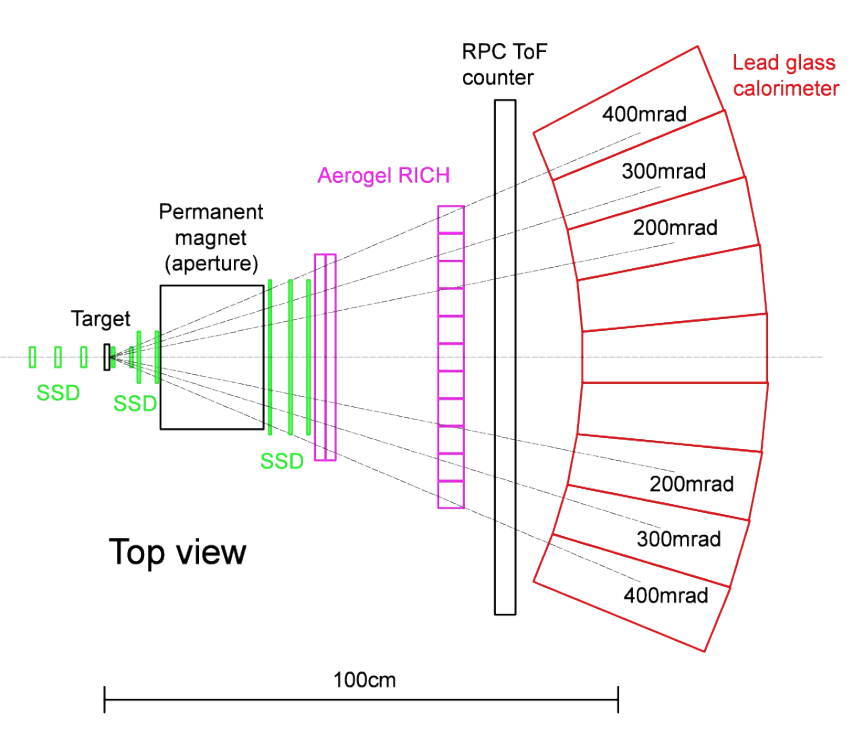
\includegraphics{./figs/EMPHATIC.png}}
\caption{Top view of the proposed EMPHATIC setup, obtained with permission from the EMPHATIC group. The different detectors in the setup are shown in different colours. The Aerogel RICH detector, RPC ToF counter, and Permanent magnet are all currently being developed.}

\label{fig:EMPHATIC}       % Give a unique label to the figure. 
\end{figure}

To obtain measurements for accelerator-based neutrino experiments, EMPHATIC will measure targets of graphite, aluminum, and iron. These targets correspond to the composition of the proposed targets, magnetic horns, and beamline components typically found in accelerator-based neutrino experiments. EMPHATIC will also measure targets composed of boron, boron nitride, and boron trioxide. Because the atmosphere is primarily composed of nitrogen and oxygen, measuring the latter two targets and removing the effects of the former will lead to estimation of hadron production in the interaction of cosmic rays in the atmosphere. 

In order to measure the production of hadrons, EMPHATIC includes four different kinds of detectors. A set of silicon strip detectors (SSDs) register the position of each particle as they pass through. A permanent magnet downstream of the target causes the trajectory of particles to curve due to the Lorentz force: the radius of the curvature depends on the momentum of the particle, so using SSDs downstream of the magnet allows for the measurement of particle momenta and trajectory. The particles then pass through an Aerogel Ring Imaging Cherenkov (ARICH) detector. As explained in Section \ref{sec:ARICH}, this detector can be used to determine a charged particle's velocity if its trajectory is known. If the velocity $\bf{v}$ and momentum $\bf{p}$ of a particle are known, then the its mass may be determined by the relativistic equation:

\begin{equation}
    \label{eq:relMass}
    m = \frac{\bf{p}}{\bf{v}}\sqrt{1-\frac{v^2}{c^2}}
\end{equation}
where $c$ is the speed of light in a vacuum. This allows for the identification of each particle.

After passing through the ARICH, particles will pass through a resistive plate chamber time-of-flight (RPC ToF) detector. This detector simply measures the time taken for a particle to travel some short distance, giving another measure of velocity. The RPC ToF has a lower resolution at the higher particle velocities measured by the ARICH detector, so these two detectors complement each other to provide a full measurement of velocities across a broad range.

After passing through the the RPC ToF, the particles strike a lead glass calorimeter, which measures the final particle energy. The lead glass calorimeter is useful for detecting any electrons or neutrons.

Currently, development is underway on the simulation and design of the ARICH detector. The ARICH detector should be able to accurately distinguish between the charged pions, charged kaons, protons, and electrons over a broad spectrum of momenta. In order to meet these goals, it is crucial that simulations be done to characterize the detector's performance and optimize the design. There are many elements of randomness in the propagation of particles through the detector, which necessitates the use of Monte Carlo simulations. 


\section{Theory}
\subsection{Cherenkov Radiation}
While the speed of light in a vacuum is fixed as $c$, when light passes through a medium with a refractive index of $n$, it will travel at the velocity $\frac{c}{n}$. When a charged particle travels through a dielectric medium at a velocity greater than the speed of light in the medium, it will emit Cherenkov radiation \cite{cherenkov}. As the charged particle travels through the medium (known as a radiator), it will displace electrons, emitting photons radially at points along the particle's path. If we define the particle velocity to be $v_p$ and $\beta = v_p / c$, then in a time $t$, the particle will travel a distance $\beta ct$. In that same amount of time, the photons emitted in the radiator have to travel a distance $(c/n)t$. The geometry of this emission is shown in in Figure \ref{fig:cherenkov}. This creates a wavefront of light emitted obeying the following relation:
\begin{equation}
    cos(\theta) = \frac{1}{\beta n}
    \label{eq:cherenkovAngle}
\end{equation}

\begin{figure}[]
\centering
\resizebox{0.35\textwidth}{!}{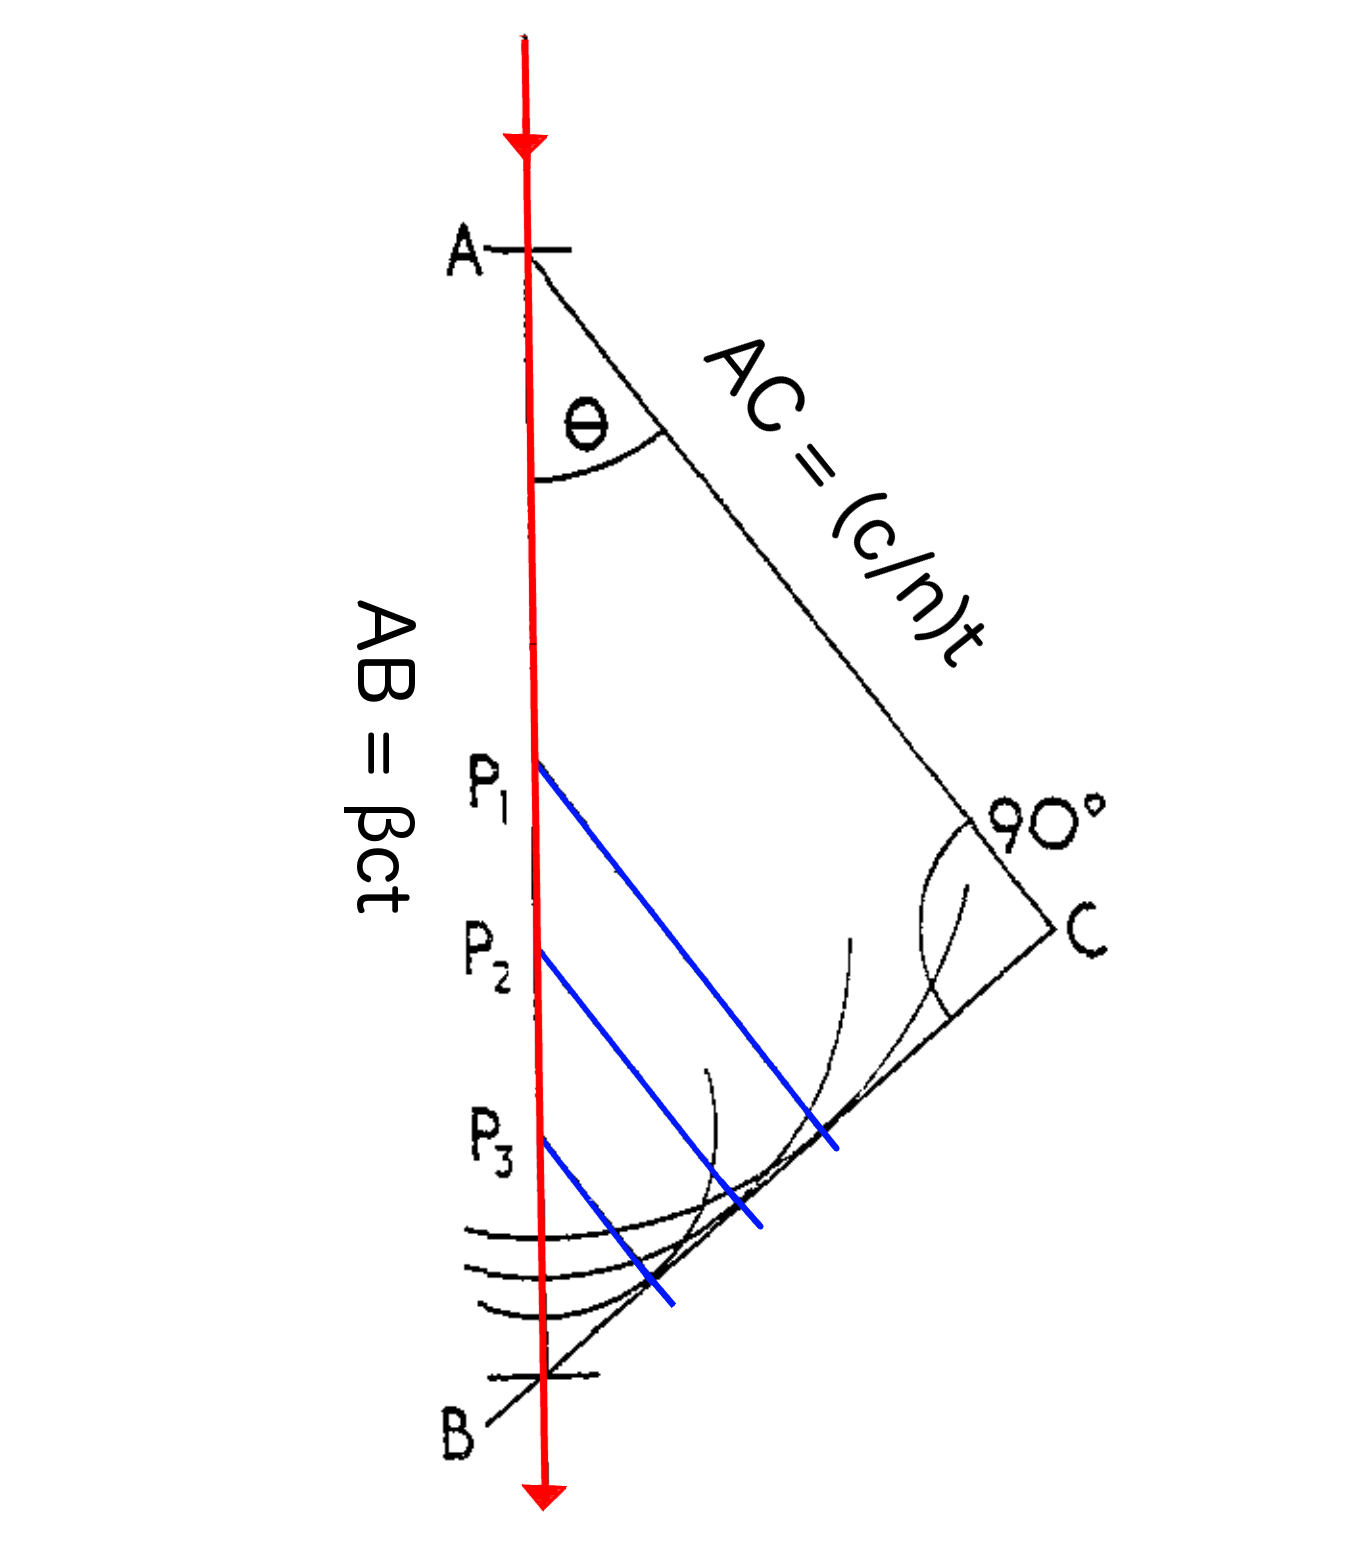
\includegraphics{./figs/cherenkovMod.png}}
\caption{Diagram showing the emission of Cherenkov radiation, adapted from \cite{cherenkov}. In this diagram, a particle travels along the vertical line from point A to point B. Electromagnetic radiation is emitted at $P_1$, $P_2$, and $P_3$, each producing one of the curves shown. It can be seen that these emissions all produce a wavefront along BC, giving a common angle of emission $\theta$.}
\label{fig:cherenkov} 
\end{figure}

This simple relation between photon angle and particle velocity is complicated by the dependency of the refractive index of a medium on the wavelength of light, which must be determined experimentally for a given radiator.

The energy emitted via Cherenkov radiation by a particle of charge $q$ as it moves a distance $dl$ is given by the Frank-Tamm formula \cite{frankTamm}:
\begin{equation}
    \label{eq:frankTamm}
    \frac{dW}{dl} = \frac{q^2}{c^2}\int_{\beta n > 1} \omega  \left(1 - \frac{1}{\beta^2n(\omega)^2}\right)d\omega
\end{equation}

In this formula, $\omega$ is the angular frequency of the light. If we neglect the frequency dependence of the index of refraction, then we can use this equation to extract the expected number of photons emitted per length $dl$ over a range of frequencies from $\lambda_1$ to $\lambda_2$:

\begin{equation}
    \label{eq:photonNumber}
    \frac{dN}{dl}  = 2\pi\alpha q^2 \left(\frac{1}{\lambda_2} - \frac{1}{\lambda_1}
    \right)\left(1 - \frac{1}{\beta^2n^2}\right)
\end{equation}

Here, $\alpha$ is the fine structure constant ($\approx \frac{1}{137}$).



\subsection{Aerogel Ring Imaging Cherenkov Detectors}
\label{sec:ARICH}
The relationship between particle velocity through a radiator and photon angle of emission (Equation \ref{eq:cherenkovAngle}) can be exploited for particle identification. An Areogel Ring Imaging CHerenkov (ARICH) detector consists of a silica aerogel radiator, and an array of photomultiplier tubes (PMTs), which can detect the Cherenkov radiation. Silica aerogel is a substance made of a network of silica (SiO$_2$) clusters interspersed with nanopores of air \cite{aerogelRefraction}. During production, the refractive index of aerogel can be precisely tuned \cite{aerogelRefraction}, and the wavelength-dependency of the refractive index is  understood \cite{aerogelWavelength}. 

High-velocity hadrons produced in the collision of the proton beam with a target will emit cones of Cherenkov radiation as they travel through the aerogel, leading to an elliptically shaped set of detected photons. With a known separation distance between the radiator and the detector, the angle of emission $\theta$ of a photon may be determined, which yields the velocity of the particle. By averaging over several photons emitted by a single particle, we can increase our angular resolution. With a thicker slab of aerogel, a charged particle travels a greater distance and is likely to emit a greater number of photons. However, this means that the point of emission of the photon can vary more, leading to lower angular resolution. To combat this, ARICH detectors can use two or more layers of aerogel with differing indices of refraction, with the layer closest to the detector having a higher index of refraction \cite{belleArich}. The photons emitted in the first layer will be emitted at a smaller angle than those from the second layer, and ultimately arrive on the same ring on the photon detector array.

The PMTs used in the detectors function by creating a rapid cascade of electrons and a corresponding signal upon being struck by a photon. Their quantum efficiencies depend on the wavelength of the incident light, and are well-characterized by the manufacturer.


\section{Details of the Proposed Calculations} 
\subsection{Initial Simulation}
\label{sec:experiment}
For my thesis project, I intend to create a fast simulation of charged particles travelling through the aerogel in the proposed EMPHATIC ARICH detector, and determine the distribution of resultant photons that strike the detector. 

These simulations will be created using \textsc{root}: a scientific computing framework based off C++ and developed at CERN \cite{root}. Our simulation will take in as input the velocity and $\theta$ and $\phi$ angles of the particle with respect to the axis of the beam. Using \textsc{root}, a vast number of particles may be simulated, whose velocities and trajectories are based off these inputs, but randomly distributed according to the resolution of the upstream particle trackers. The photons emitted by the particles travelling through the aerogel have a fixed angle $\theta$ with respect to the momentum of the particle, determined by Equation \ref{eq:cherenkovAngle}, but vary randomly with respect to their $\phi$ angle. The average number of photons emitted by each of these particles is determined by Equation \ref{eq:photonNumber}. These photons will then travel out of the aerogel and have some chance of striking the detector. The detector itself has some probability of detecting the hit, based off its efficiency. 

Once a simulation has been created to handle this procedure, it will be verified against an already-existing simulation of the full detector configuration. The full simulation is handled with \textsc{Geant4}, a C++ based software toolkit designed for Monte Carlo simulations of particles travelling through complex detector geometry  \cite{geant4}.

Once this simple simulation has been verified, the effects of photon scattering in the aerogel will be incorporated into the simulation. The transmittance of these photons through the aerogel has contributions from scattering and absorption effects, but the dominant contribution is from Rayleigh scattering \cite{aerogelRefraction}. The probability that a photon  undergoes Rayleigh scattering is proportional to $\lambda^{-4}$, where $\lambda$ is the wavelength of the light, and the angular distribution of scattered photons is proportional to $1 + \cos^2(\theta)$ \cite{rayleigh}. The known optical transmittance of the aerogel \cite{aerogelRefraction} may be fit to obtain the probability that a photon will undergo Rayleigh scattering after travelling some distance. We enhance our simulation by adding this random scattering effect to each photon: we randomly select whether the photon will have scattered at each point in its trajectory based off this probability, and generate a new $\theta$ and $\phi$ for the photon. 

After simulating thousand of particles entering the ARICH with a given velocity and trajectory, we can average over all the photons hitting the detector to get a probability distribution. An example of a probability distribution is shown in Figure \ref{fig:particleRings}. This probability distribution can then be used for particle identification.

\begin{figure}[h!]
\centering
\resizebox{0.5\textwidth}{!}{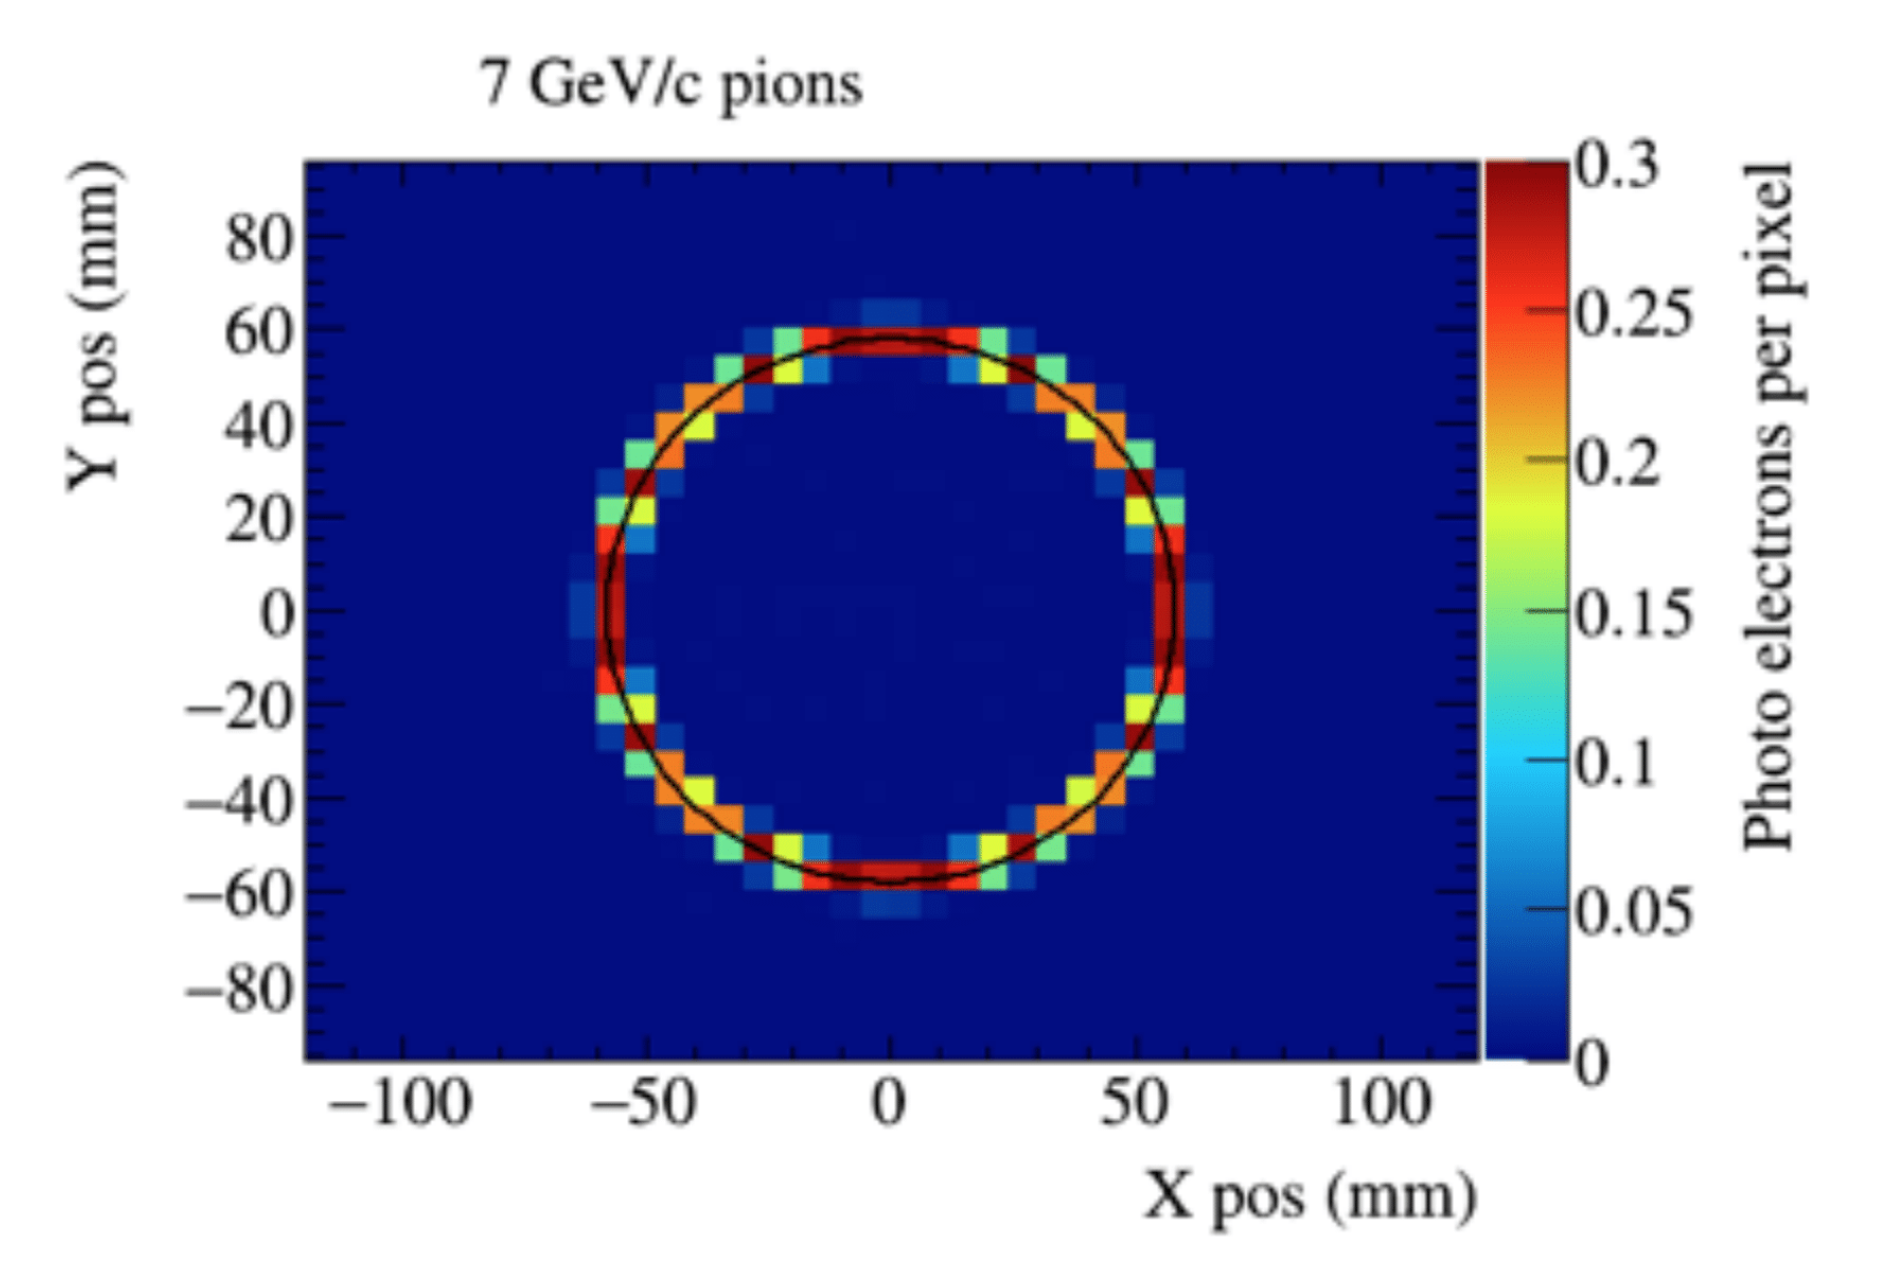
\includegraphics{./figs/particleRing.png}}
\caption{Example of the photon probability distribution on a detector plane resulting from a simulation of the photons emitted by 10,000 pions with a momentum of 7 GeV/c emitting Cherenkov radiation. The photons were simulated using \textsc{Geant4}. The figure was obtained with permission from the EMPHATIC group.}

\label{fig:particleRings}       % Give a unique label to the figure. 
\end{figure}

\subsection{Particle Identification}
\label{sec:particleIdentification}
In order to identify particles using the ARICH detector, a particle likelihood method is used \cite{richImpact, belleArich}. For this method, we take the known momentum of the particle, and use Equation \ref{eq:relMass} to determine the expected velocity for different candidate particles masses. The candidate particles of interest to the experiment are protons, electrons, pions, and kaons. For each velocity hypothesis, we run 10,000 simulations of particles moving at that velocity, with the same measured initial trajectory as input. For each pixel of the detector, this procedure will give a value $\lambda_i(\beta)$, equal to the expected number of photons striking pixel $i$ in the detector due to a particle of velocity $\beta$. 

For a given particle event, we will detect $N_i$ photons in each pixel $i$. In reality, the PMTs are only capable of registering whether or not a photon has been detected - if multiple photons strike a single pixel in a very short amount of time, it will not be able to distinguish the number detected, so we just know if $N_i = 0$ or $N_i > 0$.

The probability that zero photons strike pixel $i$ is given by the Poisson distribution for zero events:
$$ P_i(N_i=0; \beta) = e^{-\lambda_i(\beta)} $$
 The probability that one or more photons strike pixel $i$ must then be:
$$ P_i(N_i>1; \beta) = 1 - e^{-\lambda_i(\beta)} $$

By multiplying the probabilities of getting the observed result in each pixel $i$ of the detector, we calculate the likelihood for that value of $\beta$:

$$L_\beta = \prod_{i}P_i(N_i; \beta)$$

For convenience, we actually compute:
\begin{equation}
    \label{eq:loglikelihood}
    -2\ln(L_\beta) = \sum_i \ln(P_i(N_i; \beta))
\end{equation}


We compute the log-likelihood of our data matching each of particle hypothesis, and choose that which minimizes the value.

\subsection{Modifying the simulation}
After having created the simulation, I will test its ability to adequately discriminate between different particles for a broad range of particle momenta and trajectories. Following these calculations, greater realism will be added to the simulation. The specific placement of PMTs in the photon detection array can be modelled to get a more accurate picture of the detector's angular resolution and efficiency. The effects of different detector configurations may be investigated in order to get the best possible particle discrimination. 

A possible change to the detector configuration is the addition mirrors along the space between the aerogel radiator and the photon detectors. This would allow photons emitted at high angles to reflect off the mirrors and back onto the detector, increasing the total angular coverage of the detector. The effects of this addition on the detector's particle discrimination ability can also be simulated.




\section{Resources List}
Simulations will be run using the \textsc{root} framework and the \textsc{Geant4} toolkit, both of which are freely available. Large-scale simulations will be run on the TRIUMF NEUT Cluster.


\section{Planned Schedule}

\setlist{nolistsep}
\begin{itemize}
  \item \textbf{September to October:} Plan out thesis project.
  \item \textbf{November:} Familiarize myself with \textsc{root}, create fast Monte Carlo simulation of random photon emissions.
  \item \textbf{December:} Verify fast simulation against full \textsc{Geant4} simulation. Add photon scattering effects to simulation.
  \item \textbf{January:} Create more sophisticated modelling of detector with deadspace, investigate effects of pixel dimensions and positioning.
  \item \textbf{February:} Simulate the addition of a mirror to the ARICH detector and investigate effects.
  \item \textbf{March:} Write the thesis.

\end{itemize}


\section{Acknowledgements}
I would like to thank my supervisor, Dr. Mark Hartz, for all his guidance in planning out this thesis project and giving me the fantastic opportunity to work with the neutrino group at TRIUMF. I would also like to thank Dr. Matej Pavin and Dr. Akira Konaka for their helping me understand the context of the EMPHATIC experiment and for help with my computational needs. Lastly I would like to thank Dr. Rob Kiefl for his invaluable help with this proposal.


\endinput

Any text after an \endinput is ignored.
You could put scraps here or things in progress.
